\clearpage
\fancyhf{}
\fancyhead[c]{Chapter 1. General Introduction}% <- added
\fancyfoot[R]{\thepage\ifodd\value{page}\else\hfill\fi}
%\fancyhead[L]{\ifodd\value{page}\relax\else\hfill\fi Ch \thechapter}
%\renewcommand\headrulewidth{0pt}% default ist .4pt
\renewcommand{\plainheadrulewidth}{.4pt}% default is 0pt

\newpage

\noindent I urge you to look around you and observe the trees, the leaves on them, each one with a unique shape and size, isn't it? Look at the people surrounding you, how they have different skin colors, facial features, heights, voice and thoughts. Now take a look at your palm, go ahead and examine it. What do you see? Aren't all five of your fingers different from each other? If you look even closer, you would see that even the scales and crevices on your fingers are not the same. Have you ever wondered why nothing is exactly the same? Variance is an essential feature of nature; it permeates everything, from our thoughts and dreams to our language and societies. Without this diversity, life would be sterile, perhaps even impossible.

In this thesis, I have sought to understand the origins and implications of these differences at the most 
fundamental level: the neurons inside our brains. By exploring the variability among these building blocks 
of thought, ideas, dreams, language, and personality, I aim to shed light on how diversity shapes not only 
our individual experiences but also the very fabric of life. Neuroscience has long treated neurons as discrete, static ‘cell types’. But accumulating evidence shows identity lies on a continuum, is context-dependent, and heterogeneous. My aim with this thesis is to demonstrate that neuronal identity, especially the functional identity is not static but is rather dependent on the context and level of receptor specific neuromodualtion.   


\section{Neuronal heterogeneity through the lens of the past}

The mammalian brain is an extraordinarily complex organ, composed of an immense variety of neuronal cell types. This diversity is evident across multiple dimensions. Exploring this diversity has been a central tenet in neuroscience, since its inception, dating back to Ramon y Cajal (\cite{fishell2013neuron, huang2019diversity, markram2004interneurons, mukamel2019perspectives, nelson2006problem, petilla2008petilla, sanes2015types, seung2014neuronal, somogyi2005defined, yuste2020community, zeng2022cell, zeng2017neuronal}). I would like to take the reader through what I already know about neuronal heterogeneity via different modalities, 
ranging from shapes to molecular composition.    

\subsection{Morphology}

Neurons differ dramatically in their shapes and structures. Some, like pyramidal neurons, exhibit long 
apical dendrites and a characteristic triangular soma, while others, such as inter-neurons, display 
more compact and intricate branching patterns. These morphological differences are closely linked to 
the specific roles neurons play within neural circuits (\cite{liu2024neuronal}).


\subsection{Electrophysiology}

Neuronal diversity is also exhibited in the ways neurons generate and propagate electrical signals. 
Neurons exhibit distinct firing patterns, action potential shapes, spike frequency adaptation and selectivity to synaptic input. For instance, some neurons are fast-spiking, while others display spike frequency adaptation or bursting firing patterns. These electrophysiological properties are determined by the unique composition of ion channels and receptors expressed by each neuron (\cite{huang2019diversity, markram2004interneurons, mukamel2019perspectives, fishell2013neuron, masland2012neuronal, tasic2018shared, zeng2017neuronal}).


\subsection{Gene Expression}

Advances in molecular biology have revealed that neurons can be distinguished by their gene expression profiles. Single-cell RNA sequencing has enabled researchers to catalog the transcriptomes of individual neurons, uncovering a rich landscape of molecular identities. These profiles often correlate with, but are not strictly determined by, morphological and electrophysiological features (\cite{wagner2016revealing, shapiro2013single, trapnell2015defining}).


\subsection{Connectivity}

Neurons are further defined by their patterns of connectivity, both the sources of their inputs and the targets of their outputs. Some neurons form long-range projections across brain regions, while others 
participate in local microcircuits. This connectivity further defines the broader neural circuit function (\cite{Wang2021, Zhang2024, Gollo2020, Goldman2023, Tripathy2017, Sagner2019}).\\


\noindent These modalities highlight the fact that neuronal heterogeneity is multi-faceted, and challenges the notion of n-neuron types. There have been many integrative efforts that merge these different modalities. 

\subsection{Taxonomy initiatives}

In the following section I highlight the large scale efforts to study neuronal heterogeneity based on different modalities as well as the efforts towards integrating these individual modalities into a complete taxonomic picture of neuronal heterogeneity in the brain. 

\subsection{Large-Scale Taxonomy Initiatives}

In the past decade, large-scale collaborative efforts have sought to systematically map and classify the full 
diversity of neurons in the brain. Notable among these are the Allen Institute for Brain Science's Cell Types 
Program (\cite{gouwens_classification_2019,scala2021phenotypic,gouwens2020integrated}) and the BRAIN Initiative Cell Census Network (BICCN) (\cite{hawrylycz2023guide}). These projects leverage cutting-edge techniques, including high-throughput single-cell transcriptomics, large-scale electrophysiological recordings, and high-resolution imaging to build comprehensive taxonomies of neuronal types (\cite{gouwens2019classification,scala2021phenotypic,gouwens2020integrated}).

While these initiatives have greatly expanded our understanding of neuronal diversity, they often operate under the assumption that neuronal identity is static and can be captured by a fixed set of features. However, emerging evidence suggests that neuronal identity may be more dynamic and context-dependent than previously thought, raising important questions about how best to define and classify the brain's myriad cell types.

\subsection{Patch-seq}

The state of the art in recording neuronal data is a technique known as patch-seq (\cite{cadwell2016electrophysiological, fuzik2016integration}), whereby it is possible to simultaneously record morphological, electrophysiological and molecular properties of neurons. This technique is really powerful as it provides a multi-modal perspective on neuronal heterogeneity. This technique has been the linchpin in some of the biggest classification efforts such as by the Allen Brain database (\cite{gouwens2019classification,scala2021phenotypic, gouwens2020integrated}), with a multi-modal collection of more than 1900 neurons. 

In the section above, I have given an overall picture of neuronal heterogeneity through the lens of modalities such as function, physical structure and molecular composition. I have also provided an account for large-scale initiatives which aim towards creating a map of neuronal heterogeneity in the mammalian brain. In the following section, my aim is to take the reader through the concept of neuronal classification. What is the aim behind classifying neurons in cell types, the most significant classification attempts so far and the problems that still persist in this endeavor.         

\section{Neuronal Classification }

So far I have established that neuronal heterogeneity is multi-modal and the amount of data is growing exponentially. In order to make sense of these large multi-modal datasets, it is necessary to group neurons that have similar characteristics. Therefore, to manage and interpret these large, multi-modal datasets, in this thesis I adopt neuronal classification, which is the grouping of neurons with similar characteristics, as a necessary analytical framework for characterizing neuronal heterogeneity. In the following sections I will look at some of the classification approaches and discuss their limitations.  

\subsection{Traditional Classification Approaches}

Historically, neuroscientists have sought to classify neurons into discrete “types” based on intrinsic, 
relatively stable characteristics. Early classification schemes focused on observable features such as 
soma size, dendritic arborization, and axonal projections. With the advent of intracellular recording techniques, electrophysiological properties like spike shape, firing rate, and synaptic integration became central to neuronal taxonomy. More recently, molecular markers such as the expression of specific neurotransmitters, calcium-binding proteins, or transcription factors have been used to further refine neuronal classifications.

The underlying assumption in many of these approaches is that each neuron possesses a fixed functional identity: a stable set of features that persists across time and context. This has led to the widespread use of terms like ''cell type'' and ''canonical neuron'', suggesting a degree of invariance in neuronal identity. In this thesis I challenge this classic view by testing if neuronal classification depends on external factors such the somatic input distribution and neuromodulation. I have identified several limitations to these assumptions which involve the the way neurons interact with the network in which they are embedded and the recording protocols. 

I would like to mention that although, molecular markers are much stable identifiers, but molecular types and electrophysiological cell types do not always correspond together. An example of this is X94 line of Somatostatin (SST) interneuron in the mouse cortex. These cells are defined molecularly by SST expression, yet electrophysiologically they display fast-spiking, stuttering firing patterns indistinguishable from parvalbumin-positive (PV⁺) interneurons rather than the classic low-threshold–spiking Martinotti-cell phenotype of most SST neurons (\cite{scheyltjens2016current}). In the next section I will highlight the most pressing limitations which establish that the idea of static neuronal identity based on function needs a revision.  

\subsection{Limitations of Static Neuronal Classification}

In this section, we challenge the assumption of a static neuronal identity. For a long time neuronal function has been discussed in the field of neuroscience as invariant. This is can be attributed to the stimulation or input protocol used to study function of neurons. For example, since the beginning of single unit patch-clamp recordings, a static step input has been used to probe the firing rates of neurons. The following points challenge the view that functional classification of neurons is static, by highlighting problems with this assumption: 

\begin{itemize}

    \item  \textbf{The Influence of Input and Network State on Neuronal Function:} Recent experimental and computational efforts have increasingly pointed towards the idea that a neuron's functional role is not solely determined by relatively stable intrinsic properties such as morphology or gene expression, but also by the input it receives and the dynamic state of the surrounding circuit, including patterns of synaptic activity (\cite{hernath2019alternative,szabo2021conventional}), neuromodulatory influences (\cite{marder2011multiple}). Neurons operate within continuously changing environments, receiving temporally structured synaptic input that reflects sensory stimuli, behavioral demands, and ongoing internal activity. These inputs interact with intrinsic biophysical parameters in complex ways, such that the same neuron may perform different computational roles depending on the input regime or network context. Additionally, neuromodulatory systems (e.g., dopaminergic and cholinergic pathways) further reconfigure neuronal function in a cell-type- and receptor-specific manner, modulating excitability, gain, adaptation, and stimulus selectivity. This context-dependence challenges the classical view of neurons as fixed computational units. 
    
    \item \textbf{Continuous neuronal identity:} Recent large scale neuronal classification efforts have consistently shown that neurons are not discrete, modular classes but rather that their electrophysiological, molecular and morphological properties lie on a continuum (\cite{marsat2010neural,angelo2012biophysical,scala2021phenotypic}). This further complicates the effort of classifying neurons in classes. 

    \item \textbf{Limitations of Static Characterization Protocols:} Conventional approaches to neuronal classification typically rely on static stimulation protocols, such as step-and-hold current injections, to derive electrophysiological signatures. While these protocols offer insights into baseline excitability and passive membrane properties, they do not capture the complex temporal filtering or nonlinear input-output transformations that neurons perform under more realistic, time-varying conditions. In naturalistic settings, 
neuronal input is dynamic, high-dimensional, and often posses stochastic features that are absent in traditional experimental stimuli. As a result, static protocols risk underestimating or mis-characterizing the functional capabilities of neurons, potentially leading to oversimplified or misleading classifications. This disconnect highlights the need for rich stimulus paradigms, such as temporally varying current or (dynamic clamp) conductance stimuli or in vivo recordings, that better approximate the computational demands faced by neurons in situ.

    \item \textbf{Static taxonomies ignore context-dependent identity:} State of the art classification efforts assume a static functional identity of neurons. While growing body of evidence point toward a new conceptual framework in which neuronal identity is not a fixed property, but rather a context-sensitive, emergent phenomenon. If neuronal function can be reshaped by synaptic input, neuromodulatory state, and network dynamics, then neuronal identity must be understood as fluid and multidimensional, rather than static and categorical. This dynamic view aligns with recent findings showing that neurons shift the cell-class (\cite{andriatsilavo2025toward}) they belong to depending on the input stimulus or modulatory condition (\cite{szabo2021conventional,hernath2019alternative}). It also suggests that functional heterogeneity in neural populations is not simply stochastic noise, but may reflect adaptive specialization to a range of computational roles. In this thesis, I explore this emerging view by analyzing how neurons reorganize their functional attributes under different input regimes and neuromodulatory conditions, using high-dimensional clustering and integrative analysis across multiple feature domains. This work contributes to a growing shift in neuroscience: from static taxonomies to dynamic, functionally grounded models of neuronal identity. 
    
    \item \textbf{Failure to capture the high-dimensional functional space of neurons:} The functional space of neurons is high-dimensional, this is due to the fact activity of neurons depends on the activation/inactivation of different ion-channels (\cite{fyon2024dimensionality}), which in turn are modulated by the context (synaptic input) they receive. This can be summarized by passive properties such as resistance, capacitance, etc. Furthermore, neurons filter inputs across temporal dimensions to elicit spikes, drawing on a high-dimensional input space. This increases the dimensional complexity of their input–output transformations (\cite{y2003computation}). Yet, most electrophysiological classifications studies only consider one feature at a time. This leads to an incomplete picture of functional heterogeneity. As I have discussed before, stimulus protocols have a strong role to play in features that can actually be extracted. For example, synaptic-type inputs drive neuronal firing across a broader range of membrane potentials and spike thresholds than step current stimulation (\cite{szucs2015differential}). Therefore, properties related to action potential are a function of the input protocol. Clustering based on these features typically involves looking at a low dimensional (1-3 dimensions) feature space (\cite{druckmann2013hierarchical}) or a projected space using a method such as K-means clustering method. This approach underestimates the rich functional space in which neurons function and thus clustering based on functional properties needs a method that utilizes multiple features pertaining to function simultaneously and provides a rich overview of functional heterogeneity. 
    
    \item   \textbf{No consensus on properties that are the most informative about heterogeneity:} While neurons have been categorized based active and passive features, there is no consensus on attributes or a set of attributes that are the most informative about heterogeneity. Identifying the attributes that capture the most relevant heterogeneity is essential, because clustering on the wrong or incomplete feature sets leads to unstable or misleading classifications. While most classification studies (\cite{connors1990intrinsic,petilla2008petilla,gouwens2019classification,gouwens2020integrated,scala2021phenotypic}) focus on passive properties such as capacitance or conductance of the cell or active properties such as firing rates and inter-spike intervals, there are no studies that compare the estimate of neuronal heterogeneity based on different sets of properties and provide a consensus for the field. Moreover, the properties extracted are limited by the stimulation protocol. For example it is not possible to estimate the linear input-filter of a neuron via a step input protocol, and thus it requires a white noise based stimulation protocol. Therefore, it is essential to first compare input protocols based on their viability, and establish the input protocol that is most suitable for studying a neuronal population. It is only then we can compare properties extracted for that protocol in order to provide a consensus.  
\end{itemize}

\noindent   The limitations listed above show that assuming a static neuronal identity is restrictive, it gives an incomplete picture of a rich high-dimensional and dynamic functional space in which neurons reside. Therefore, a new method is required to ascertain the high dimensional and dynamic nature of neuronal function by taking into account the input context and functional properties used to study function. 

So far I have highlighted the limitations of input protocol and the lack of consensus in determining the most informative properties to study functional heterogeneity, but a very important topic still remains to be discussed and that is neuromodulation. Neurons contain ion channels in their membranes, which are susceptible to modulation via specific receptor activation molecules. These neuromodulators have a strong effect on the activity of neurons, they can suppress or enhance firing of a neuron. Therefore, it is important to study how neuromodulation affects neuronal function and classification. The following section discusses what we currently know about neuromodulation in terms of their effect at a single neuron level.   

\section{Neuromodulation: Reconfiguring Neural Computation}

Neuromodulatory systems, particularly those involving dopamine and acetylcholine play a critical role in shaping brain states associated with attention, learning, memory, and pathology (\cite{dalley2004cortical,hasselmo2006cholinergic,sarter2009phasic}). Rather than directly triggering spikes, these modulators reshape how neurons respond to input, modulating intrinsic excitability and synaptic integration (\cite{dascal2001ion,seong2012d1,cousineau2020dopamine,bargmann2012beyond, marder2012neuromodulation,taghert2012peptide}). Their effects are often receptor and cell-type-specific, suggesting a finely tuned mechanism for reconfiguring the computational landscape of cortical networks.

Despite extensive behavioral and molecular work (\cite{nadim2014neuromodulation,mccormick2020neuromodulation,avery2017neuromodulatory}), the functional impact of neuromodulation on neuronal computation remains poorly understood, especially at the level of high-dimensional feature interactions. Are neuromodulatory effects isolated to individual electrophysiological features, or do they act in a coordinated manner to restructure how neurons encode information?

The following points summarize the gaps of what remains to be understood in regards to the effect of neuromodulation, specifically dopaminergic and cholinergic modulation, on single neurons: 

\begin{itemize}
    \item \textbf{Effect of neuromodulation on computation} Much is known (\cite{dalley2004cortical,hasselmo2006cholinergic,sarter2009phasic,nusser2009variability}) about molecular and excitability changes caused by dopamine and acetylcholine modulation in single neurons; it is still unclear how this alteration in excitability changes what neurons compute. Since neurons relay information within a network, it is unclear how dopamine and acetylcholine, change information transfer in neurons. Since the activity of individual neurons determine the state of a network, it is clear that understanding alteration in transferred information in single neurons due to neuromodulation would explain a lot about the properties of cortical circuits. 

    \item \textbf{Heterogeneous modulation in neuronal population} A given population of neuron comprises of individuals or sub-groups of neurons that differ from each other in terms of their shape and ion-channel type and distribution. It is still unclear how this individual variability manifests itself on a circuit scale. While it is known that this heterogeneity provides flexibility to the circuit (\cite{wu2025neural,hutt2023intrinsic}), the effect of neuromodulation on this individuality is still unclear. More precisely, it is unknown if all functional properties are altered uniformly or if there exists a heterogeneity in terms of properties that are altered due to specific modulation and what population level effects of neuromodulation are. 

    \item \textbf{Reconfiguration under the influence of dopamine and acetylcholine} Most studies that focus on neuromodulation of individual neurons, focus on how individual active or passive properties such as firing rate or conductance are altered due to a specific receptor activation. While it is important to study how individual properties are altered due to neuromodulation, it is also important to study how the high-dimensional functional space of neurons is altered due to neuromodulation. This requires looking at the correlation structure between active and passive properties of neurons and how this correlation structure changes due to neuromodulation.
\end{itemize}

Up to this point, I have examined neuronal heterogeneity from multiple angles and the challenges of classifying single neurons, including the role of neuromodulation at the cellular level. However, focusing on single neurons provides only a limited perspective: what ultimately matters is how heterogeneity shapes computation at the network level. Since it is not currently feasible to study this directly in large cortical circuits, we turn to artificial neural networks, where parameter variability across individual units can be systematically explored. The next section sets the context for this approach.   
          
\section{Effect of Timescale Heterogeneity in Artificial Systems}

Biological neural systems are composed of heterogeneous computational units (individual neurons) with diverse intrinsic properties (\cite{koch1999complexity}). This diversity has been shown to support critical functions such as motor control (\cite{cavanagh2020diversity}) and memory formation (\cite{mcnaughton2006path, hasson2008hierarchical, chu2020long}). While this fact is well-accepted in neuroscience, most artificial neural networks continue to be designed with homogeneous units. Although some biologically inspired neural networks such as spiking neural networks have shown benefits of intrinsic heterogeneity (thresholds, timescales, and connectivity) on variety of tasks, more specifically on encoding and memory task (\cite{gast2024neural,perez-nieves_neural_2021,chakraborty_heterogeneous_2022,zeldenrust_efficient_2021, mejias_optimal_2012,tripathy_intermediate_2013,landau_impact_2016,doty_heterogeneous_2021,duarte_leveraging_2019}). These results suggest that incorporating timescale diversity improves computational performance. 

Simpler models, such as Recurrent Neural Networks (RNNs), which possess temporal memory, have been proposed as functional analogs to biological circuits (\cite{sussillo2014neural}). One popular subclass, Reservoir Computing (RC) (\cite{jaeger2001echo,maass2002real}) networks, or Echo State Networks (ESNs) (\cite{jaeger2001echo,jaeger2001short,jaeger2003adaptive}), have been demonstrated to have the capacity to solve tasks requiring short-term memory (\cite{jaeger2001echo}). However, these networks are typically built with nodes consisting of identical intrinsic parameters and lack the diversity observed in biological systems. Studying heterogeneity in an RC framework provides a useful middle ground over spiking neural networks: we can examine the computational role of intrinsic heterogeneity by varying the timescales of individual units, which is the only intrinsic parameter governing the dynamics of individual units, in a controlled and analytically tractable setting, while avoiding the training difficulties of more biologically detailed spiking networks. This makes RC an ideal testbed for rapid exploration of how heterogeneity contributes to network-level computation. 

Recent studies have introduced architectural temporal heterogeneity between nodes in ESNs, wherein signal propagation delays between nodes are distributed based on their spatial distances. These networks are called Distance-based Delay networks (DDNs). Objectively, DDNs have been shown to outperform classical ESNs on memory and chaotic time-series tasks (\cite{iacob2022distance, soriano2014delay}). However, heterogeneity is still embedded in network connectivity and the distributed delays between individual units in case of DDNs, not in the intrinsic properties of individual units. Even though topological heterogeneity has been shown to be beneficial, it still remains unclear how intrinsic temporal heterogeneity such as modular variability (e.g., groups of neurons sharing a timescale distribution) in decay rates of individual units in the network or integration time constants across individual units influences network performance. 



\section{Research Objectives and Key Questions}
So far I have explained various facets of neuronal heterogeneity, the current understanding and limitations of static protocol to study functional heterogeneity. I have also touched upon neuronal heterogeneity considering the effect of neuromodulation, how functional and computational properties of individual neurons and networks are known to be affected by it. And finally, I have laid the ground work for timescale heterogeneity in artificial systems such as RC systems. In the next section we synthesize the research gaps and formulate research objectives based on them. Taking the central tenet, which is neuronal heterogeneity into account, this thesis addresses three overarching questions:

\begin{enumerate}
  \item \textbf{How does input context influence functional classification of neurons and which feature(s) are the most informative about neuronal heterogeneity?} \\
In Chapter 2, using existing data (see below) I demonstrate that neuronal identity is not static, but input-dependent, with classification outcomes varying significantly under dynamic versus static stimuli. This challenges the notion of fixed cell types determined on the basis of electrophysiological features and highlight the role of stimulus structure in shaping neural function. Furthermore, I extract and compare attributes from the neural recordings under a dynamic input stimulus in-order to identify the functional feature that is the most informative about heterogeneity.   

  \item \textbf{How does neuromodulation alter the functional landscape of neurons?} \\
In Chapter 3, using part of the same preexisting data I explore how activation of dopaminergic (D1-R, D2-R) and cholinergic (M1-R) receptors reconfigure information encoding, shifting the correlation structure between feature domains. I show that neuromodulatory effects are highly cell-type and receptor-specific, modulating not just individual functional attributes but also their coordination.

  \item \textbf{Can intrinsic timescale heterogeneity improve performance and memory in reservoir computing systems?} \\
In Chapter 4, I move from data analysis to modeling, using a reservoir network to study the effect of intrinsic heterogeneity. For this, I design 4 different variants of ESNs and DDNs with varying levels of timescale heterogeneity, which is the only intrinsic parameter governing the dynamics of individual units, and optimize them to perform NARMA-30 and Mackey-Glass benchmark tasks. I study the effect of the designed heterogeneity on task performance, stability, representation and memory capacity. I show that an intermediate level of heterogeneity is optimal for solving the two benchmark tasks, suggesting that the level of heterogeneity required for optimal performance is task dependent.     
  
\end{enumerate}


\section{Experimental Framework and Approach}

For answering the first two research questions stated above, this thesis utilizes single unit in-vitro patch clamp recordings form the somatosensory cortex layer 2/3 (\cite{da2018databank}). These recordings were performed in tandem, first using a static step and hold input protocol, followed by a frozen noise protocol (see below) (see Fig. \ref{fig:input_protocol}). Within each input protocol, neurons were first recorded in a vehicle control (artificial cerebral spinal fluid - aCSF) condition and a drug condition, where a specific receptor agonist is added to the bath and the recording is performed again. Sometimes multiple control and drug trials are recorded for a single neuron.   

\subsection{Input Protocols }
\begin{figure}
    \centering
    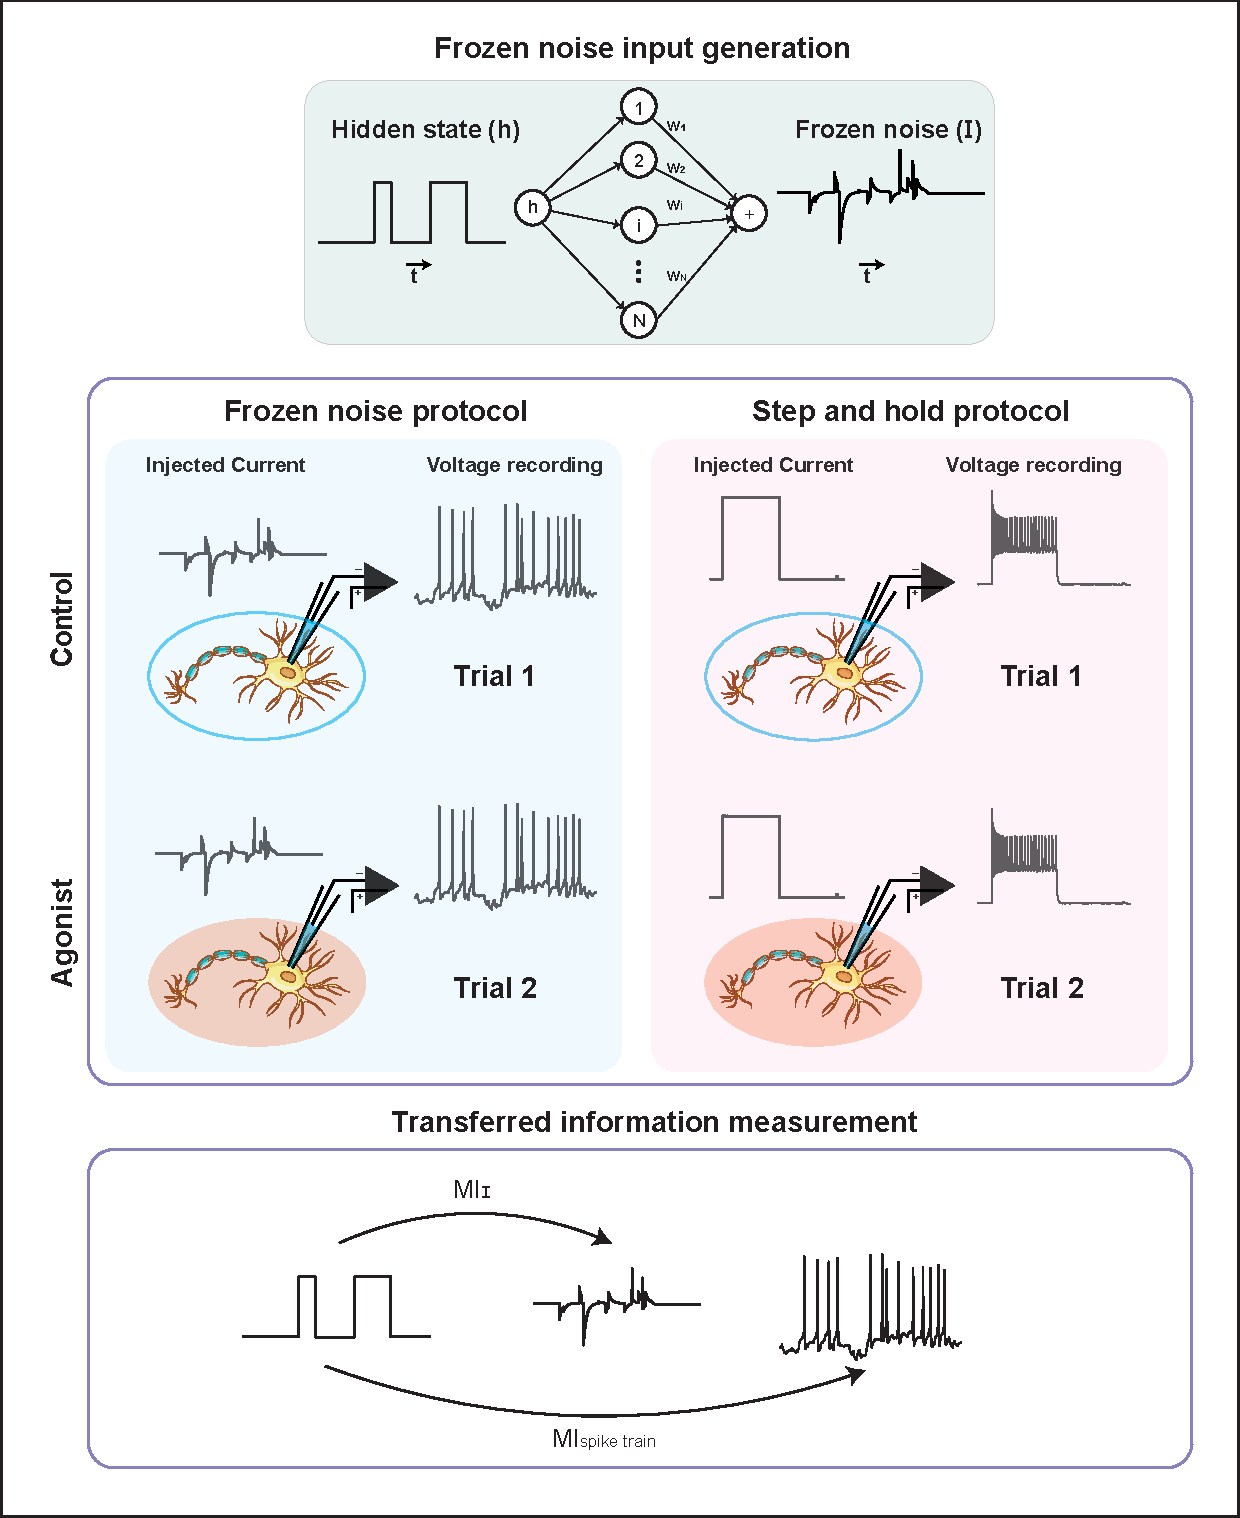
\includegraphics[width=\linewidth]{Figures/Intro/input_protocol.pdf}
    \caption{\textbf{Data collection and input protocol} the top figure shows the process of input generation using the hidden state and an artificial neural network. The middle figure shows the recording process, the neurons are recorded first in control condition using the frozen noise and step and hold inputs respectively, and then a specific receptor agonist is added, and the recording is repeated again. The bottom figure shows the procedure for measuring transferred information. Mutual information is measured between the hidden state and the input as well as between the hidden state and the spike train. } 
    \label{fig:input_protocol}
\end{figure}

\subsubsection{Step and Hold}

The step-and-hold protocol is a widely used electrophysiological method for characterizing neuronal properties through controlled current injections. In this protocol, a neuron's membrane potential is maintained at a baseline value (commonly around -70 mV), and then a series of incremental current steps are injected, each lasting for a fixed duration, typically 500 ms with recovery periods (e.g., 5.5 seconds) between steps. The current amplitude is increased in defined increments (e.g., 40 pA per step), allowing researchers to observe how the neuron responds to increasing levels of depolarizing input, including changes in firing rate, spike threshold, and other action potential characteristics. This approach enables the classification of neurons (such as distinguishing between bursting, fast-firing and regular-firing types) and the assessment of properties like maximum firing frequency, spike latency, and after-hyperpolarization. The step-and-hold protocol thus provides a standardized way to probe intrinsic excitability and firing dynamics, serving as a foundational tool in cellular neurophysiology. 

\subsubsection{Frozen Noise}

The frozen noise protocol (\cite{zeldenrust2017estimating}), is a method designed to quantify the mutual information between a neuron's input and its spike train output in electrophysiological experiments. This protocol generates a time-varying input current by simulating the activity of a presynaptic neural network of 1,000 neurons, each firing Poisson spike trains in response to a binary "hidden state" (a Markov process representing the presence or absence of an external stimulus). 
The injected current is "frozen", meaning the same input sequence is used across trials or conditions, enabling a direct comparison of neuronal responses. By analyzing how the recorded neuron transforms this structured input into spikes, researchers can calculate the information-theoretic relationship between the hidden state and the output spike train. 
This approach overcomes limitations of traditional step-and-hold protocols by mimicking naturalistic synaptic input patterns while maintaining experimental control, allowing efficient bias-free information quantification with short (6 minutes) recordings. The protocol's output includes the injected current trace, hidden state time series, and the neuron's voltage response, facilitating both forward modeling of neuronal dynamics and reverse-engineering of coding principles. 

\subsection{Extracted features}

A part of the first research objective is to identify the most informative attribute(s) (see above) when neurons are stimulated with a dynamic input protocol. In order to create a framework towards providing a consensus about the most informative attribute(s), I extracted neuronal function attributes and categorized into four distinct sets. This grouping is performed in order to capture distinct facets of neuronal function. This includes attributes ranging from passive properties to feature selectivity. Listed below are the attribute sets extracted from recordings stimulated with a dynamic input:
\begin{itemize}
  \item \textbf{Action Potential (AP) attributes --} This attribute set contains 22 features related to action potential shape and dynamics with their descriptive statics.  
  \item \textbf{Passive Biophysical (PB) attributes --} This attribute set contains 6 features related to passive properties such as membrane capacitance.   
  \item \textbf{Adaptation Currents (AC) --} This attribute set is a curve that captures the adaptation dynamic after an action potential.   
  \item \textbf{Input Feature Selectivity via Spike Triggered Average (STA) --}. This is an attribute set that captures the input feature selectivity of neurons. 
\end{itemize}

An overview of the feature extraction and analysis pipeline is shown in Fig. \ref{fig:feature_extraction}. To dissect how neuronal encoding depends on input protocol and neuromodulatory state, I applied three complementary analyses. First, unsupervised high-dimensional clustering (\cite{lee2021non}) was used to assess how neurons group under different input protocols and across drug versus control conditions. Second, cosine similarity analysis quantified the degree of heterogeneity within each attribute set. Third, Multi-set Correlation and Factor Analysis (MCFA; \cite{brown2023multiset}) compared relationships across attribute sets to identify which features were most informative about heterogeneity and how different functional domains covary. Together, these analyses reveal both within-set variance and cross-set coordination, providing a system-level view of functional reconfiguration. 

\begin{figure}
    \centering
    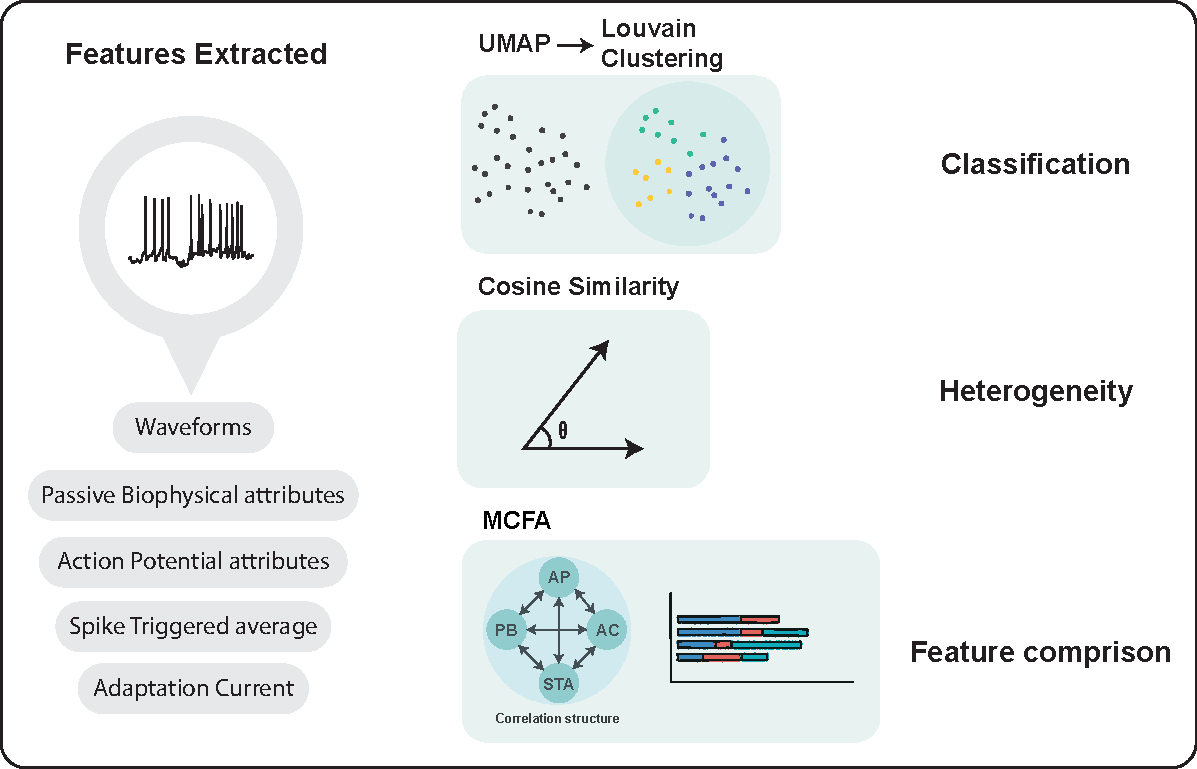
\includegraphics[width=\linewidth]{Figures/Intro/analysis_tools.pdf}
    \caption{\textbf{Overview of extracted features and analysis tools}}
    \label{fig:feature_extraction}
\end{figure}

\subsection{Network Design}
In order to study the effect of heterogeneity of intrinsic properties, in this case the time constant of individual units, on performance, memory and stability. I chose time constant as the intrinsic parameter of interest because it directly controls the temporal scale and memory of each unit, a crucial mechanism for capturing multi-timescale dependencies observed in complex dynamical systems and biological neural networks. I designed four different heterogeneity types for ESNs and DDNs. These configuration capture different levels of heterogeneity. I tested network wide heterogeneity and contrasted it with the network divided into modules or clusters, with each cluster having its own parameter sampled from a distinct distribution. The designed network configurations are summarized as following: 
\begin{enumerate}
    \item \textbf{Homogeneous Network}: All units share a single decay (time constant) parameter.
    \item \textbf{Homogeneous Cluster}: The ESN/DDN is divided into clusters, each cluster with its own fixed decay parameter.
    \item \textbf{Heterogeneous Network}: Each unit samples its decay from a shared distribution.
    \item \textbf{Heterogeneous Cluster}: Each cluster samples decay parameters from different distributions.
\end{enumerate}

I also wanted to test if task complexity decides the requirement for the optimal level of network heterogeneity. I tested these networks on two benchmark tasks, namely NARMA-30 and Mackey-Glass tasks:
\begin{itemize}
    \item \textbf{NARMA-30}: A nonlinear auto-regressive moving average task designed to test long-range memory and nonlinear dynamics. 
    \item \textbf{Mackey-Glass}: A chaotic time-series prediction task that evaluates a network's ability to generate stable yet complex temporal outputs.
\end{itemize} 

I trained these ESNs and DDNs on the two tasks mentioned above and study the effect of intrinsic heterogeneity on stability, memory capacity and dimensionality of these networks. 

\section{Summary and Outlook}

This introduction has outlined the motivation and rationale for investigating neuronal identity based on function through the dual lenses of input-dependence and neuromodulatory flexibility. Traditional classification approaches, though informative, fall short in capturing the high-dimensional, dynamic nature of neuronal computation. By leveraging state of the art patch clamp recordings done using frozen noise protocols, extracting high dimensional electrophysiological features from these recordings, and using modern unsupervised analysis techniques, this thesis proposes a data-driven framework to redefine neuronal identity as an emergent, context-sensitive construct. Also, using the extracted features, this thesis provides a comparative framework towards a consensus about functional heterogeneity, which is further useful for clustering. Finally, this thesis investigates the computational implications of intrinsic heterogeneity by modeling structured diversity in artificial reservoir systems. The following chapters present experimental results and theoretical insights that collectively support this paradigm shift.

\section{Thesis Structure}
\begin{itemize}
  \item \textbf{Chapter 2}: Neuronal Identity is Not Static: An Input-Driven Perspective \\
  Demonstrates how different stimulation protocols yield distinct classifications of neurons, showing that neuronal identity is dynamic and shaped by input. It also provides a comparison between attribute sets for understanding the most informative feature for functional heterogeneity. 

  \item \textbf{Chapter 3}: Neuromodulatory Control of Cortical Function \\
  Examines how neuromodulators reshape the computational roles of neurons, altering both encoding capacity and feature interdependence.

  \item \textbf{Chapter 4}: Timescale heterogeneity in reservoir computing \\   
    Analyzes the effect of timescale heterogeneity on task performance of ESNs and DDNS, showing that moderate timescale heterogeneity improves the performance of networks with moderate heterogeneity relative to networks without it .  

  \item \textbf{Chapter 5}: General Discussion and Future Directions \\
  Integrates findings presented in this thesis, discusses implications for neuroscience and artificial neural networks, and proposes directions for future research.
\end{itemize}


\newpage
\begin{spacing}{1.0} % Set the line spacing to single spacing
\fontsize{8pt}{8pt}\selectfont
\bibliographystyle{apalike}
\renewcommand{\bibname}{References}
\bibliography{All_bibtex}



\end{spacing}
